\section{Scale-space blob detection [45 points]}




\begin{figure}[h]
\centering
\begin{tabular}{cc}
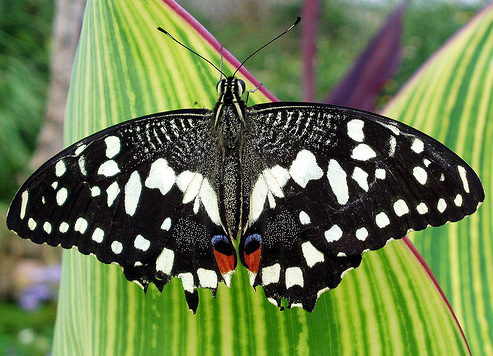
\includegraphics[width=0.4\linewidth]{./fig/butterfly.jpg} &
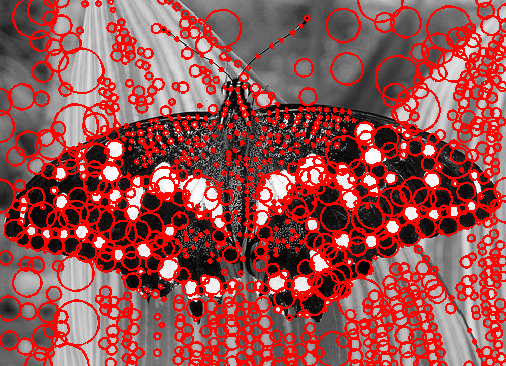
\includegraphics[width=0.4\linewidth]{./fig/butterfly.png} \\
\end{tabular}
\caption{\label{fig:blobs} Scale-space blobs detection}
\end{figure}




In this homework you will implement a simple panoramic image stitching algorithm. The first part is to detect blobs as keypoints. The algorithm is outlined as follows:


\begin{enumerate}
\item Build a Laplacian scale space, starting with some initial scale and going for n iterations:
\begin{enumerate}
\item Filter image with scale-normalized Laplacian at current scale.
\item Save the square of Laplacian response for current level of scale space.
\item Increase scale by a factor k.
\end{enumerate}
\item Perform non-maximum suppression in scale space.
\item Display resulting circles at their characteristic scales for points above a threshold.
\end{enumerate}


\paragraph{Test images.} There are four images in the folder \cmd{data/blobs} to test your code. Fig.~\ref{fig:blobs} provides the output of "butterfly" example as a reference to debug your code. Keep in mind that your output may look different depending on your threshold, range of scales, and other implementation details.


\paragraph{Running the code.} Start from the entry code \cmd{evalBlobsDetection}. It calls the dummy implementation of \cmd{detectBlobs} and draws the blob with \cmd{drawBlobs} as Fig.~\ref{fig:dummy}. You will need to install \cmd{scikit-image} and \cmd{OpenCV} by \cmd {conda install scikit-image} and \cmd{conda install -c menpo opencv}. You need to implement the function in \cmd{detectBlobs} which outputs a $n \times 4$ matrix with a blob in each row as (x, y, radius, score). 


\begin{figure}[h]
\centering
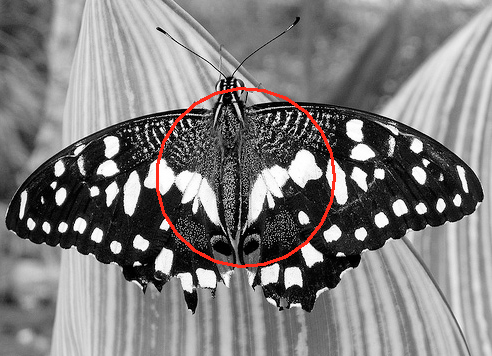
\includegraphics[width=0.3\linewidth]{./fig/butterfly-dummy.png} 
\label{fig:dummy}
\caption{\label{fig:dummy} Output of running the default implementation of evalBlobsDetection}
\end{figure}


The following are the hints to implement the function:


\begin{itemize}
\item Don't forget to convert images to gray-scale and double. 
%(\cmd{rgb2gray} command) (\cmd{im2double}).
\item For creating the Laplacian filter, you may use the function \cmd{scipy.ndimage.generic\_laplace} or \cmd{cv2.Laplacian}. Pay careful attention to setting the right filter size.
%\cmd{fspecial} 
\item You have to choose the initial scale, the factor $k$ by which the scale is multiplied each time, and the number of levels in the scale space. I typically set the initial scale to 2, and use 10 to 15 levels in the scale pyramid. The multiplication factor should depend on the largest scale at which you want regions to be detected.
%\item You may want to use a 3D array to represent your scale space. It would be declared as:


%\begin{center}
%\textit{scaleSpace = zeros(h,w,n); \% [h,w] - dimensions of image, n - number of levels in scale space}
%\end{center}


%Then \textit{scaleSpace(:,:,i)} would give you the i'th level of the scale space. Alternatively, if you are storing different levels of the scale pyramid at different resolutions, you may want to use a cell array, where each "slot" can accommodate a different data type or a matrix of different dimensions. Here is how you would use it:
%\begin{center}
%\textit{scaleSpace = cell(n,1); \%creates a cell array with n "slots"} \\
%\textit{scaleSpace\{i\} = myMatrix; \% store a matrix at level i}
%\end{center}


\item A point is the local maximum if it is higher than all its neighbors (each point has 26 neighbors in 3D). 
%You may find functions \cmd{nlfilter}, \cmd{colfilt} or \cmd{ordfilt2} useful for doing non-maximum supression in Matlab. 
In Python, you might want to use \cmd{scipy.ndimage.filters.generic\_filter} in your implementation.


\item You also have to set a threshold on the squared Laplacian response above which to report region detections. You should play around with different values and choose one you like best.


\item To display the detected regions as circles, you can use the \cmd{drawBlobs} function. You should display the highest scoring 1000 detected blobs for each image. If your code returns fewer than 1000 blobs then you may have to lower your threshold. Don't forget that there is a multiplication factor that relates the scale at which a region is detected to the radius of the circle that most closely approximates the region.
\end{itemize}


\subsection{What to submit}
To get full credit of this part, you have to
include your implementation of \cmd{detectBlobs} and include the results of given test images under \texttt{data/blobs}.






